\subsection{Lecture de tension de la batterie}
	\paragraph*{}
	Pour valider qu'il n'y ait pas d'erreur avec la lecture de tension des modules, on compare leur somme avec la tension de la batterie. Si l'écart est trop grand entre les deux valeurs, une défaillance pourrait s'être produite. La mesure de la tension de la batterie sert également à estimer l'état de la charge et vérifier la tension durant la précharge. 
	
	\paragraph*{}
	Tout d'abord, puisque cette lecture est effectuée sur de la haute tension, il est préférable d'isoler le circuit. De plus, chaque polarité de la batterie a son propre connecteur pour éviter l'inversement de polarité. Ils sont également distancés pour empêcher un arc électrique lors de la connexion ou la déconnexion des connecteurs.
	
	\paragraph*{}
	Ensuite, toujours sur la partie isolée, un simple diviseur de tension vient réduire la haute tension. On suppose que la plage de la haute tension est de 0-200 V, pour la réduire à une plage de 0-2 V.
	
	\paragraph*{}
	Une fois la tension réduite, on isole le signal avec un détecteur de tension de précision, isolé de façon optique. Le détecteur produit ensuite sur le côté non-isolé une tension proportionnelle à son alimentation de sortie.
	
	\paragraph*{}	
	Puisque l'alimentation à l'entrée du détecteur doit être isolée, on utilise un convertisseur de courant continu. Le 12V de la partie non-isolée convertira à 5 V sur la partie isolée pour alimenter le détecteur.
	
	\paragraph*{}	
	Pour que le microcontrôleur puisse lire la tension avec son ADC, il faut convertir la tension de sortie du détecteur à 3.3 V. Pour ce faire, on utilise un amplificateur opérationnel avec un gain ajusté pour convertir une plage de 0-5 V à 0-3.3 V.
	
	\begin{figure}
		\centering
		\fbox{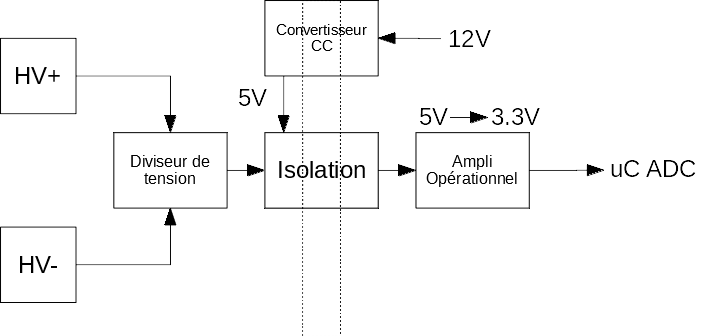
\includegraphics[width=0.7\linewidth]{Images/SchemaLectureTension}}
		\caption{Schéma du circuit de la lecture de tension de la batterie}
		\label{fig:schemalecturetension}
	\end{figure}
	
	\begin{table}[H]
		\centering
		\caption{Sélection des composantes du lecteur de tension de la batterie}
		\label{SelectionSenseVoltageBat}
		\begin{tabular}{|p{3cm}|p{3.5cm}|p{6cm}|p{1.5cm}|}
			\hline
			\textbf{Composantes} & \textbf{Manufacturier} & \textbf{Description} & \textbf{Prix}
			\\ \hhline{|=|=|=|=|}
			ACPL-C87A-500E & Broadcom Limited & détecteur de tension de précision & 10.35 \$	\\ \hline
			LMV321RILT & STMicroelectronics & Amplificateur opérationnel tout usage & 0.65 \$	\\ \hline
			NCS1S2405SC & Murata Power Solutions Inc. & convertisseur de courant continu & 12.29 \$	\\ \hline
		\end{tabular}
	\end{table} 